%%%%%%%%%%%%How does a GPS work and draw the state diagram for the GPS.Describe the different alternatives for measuring power consumption of a GPS%%%%%%%%%%%%%%%%%%%%%%%%%


\chapter{Background}

okai lets do tthis

\subsection{GPS}
The Global positioning system is a space based radio navigation system developed by the Unites States Government.  The system provides both timing and geolocation information to a GPS receiver anywhere on the Earth.  The system is not influenced by the number of receivers and can therefore serve an unlimited amount of users. The GPS system can deliver a position which is accurate within 22 meters horizontally if only one receiver is used. If multiple receivers is used positioning accuracy level of the order of a subcentimeter to a few meters can be obtained \cite{GPS}.

GPS consists of 24 satellites that are arranged so that minimum four satellites is visible anywhere on the earth. Each satellite continuously broadcasts a signal composed of two carriers, two codes and a navigation message which contains the coordinates of the satellites.  If the distance between three satellites are known, the location of the receiver can be determined by measuring the angles with the respect of the each satellite.  Figure \ref{fig:GPS} shows the resection that is used by the satellites to determine the position.\\

\begin{minipage}[t]{0.8\textwidth}
    \centering
    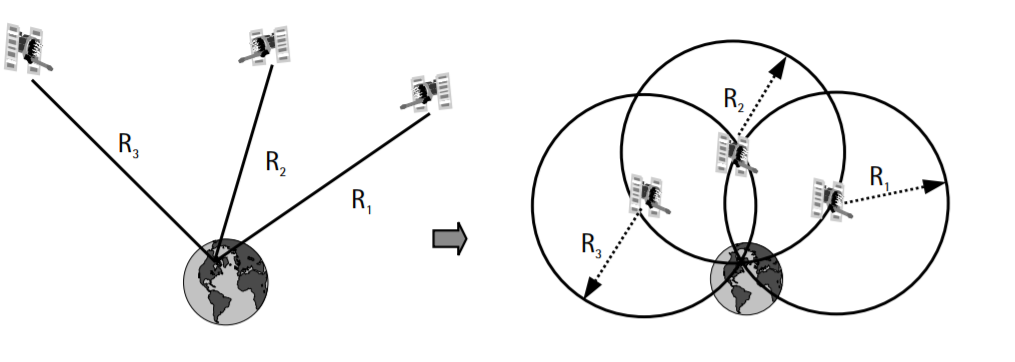
\includegraphics[width=0.8\textwidth]{Images/gps.PNG}\\
    \caption{\ref{fig:GPS} : Resection used by the satellites to determine the position}
    \label{fig:GPS}
\end{minipage}
\\

  GPS needs an additional satellite to account for the clock offset. A method for determining the velocity of a GPS is by estimating the Doppler frequency of the received signal. The satellites broadcasts two types of navigation messages. The Almanac contains course date for all the Space Vechicles(SV). Each SV broadcast this for ALL SVs. The Almanac is valid for up to several months. The Ephemeris contains precise information about orbital position and clock correction is only valid for up to 30 minutes. Both of these are critical for getting a GPS fix, and they are often one of the time limiting factor for getting the position. 
  An outdated almanac or ephemeris can cause a slow start, this can happen if the receiver hasn't been used in a while, a cold start is done or the receiver has traveled a far distance while turned off.

\subsection{Measuring power consumption}

\subsubsection{Shunt resistor}
\subsubsection{Simulating GPS with a Model}
\subsection{Code analysis}
